% Standalone 6.3 draft; historical CSV analysis only, not included in thesis.tex.
\section{多轮对抗优化实验}
\label{sec:ch06_multi_round_adversarial}

前述对照区分了判别输入与梯度路径，但尚未回答：判别器适应已有生成结果后，再更新生成场，能否持续改善迁移质量。为建立可比较的起点，先对冻结候选开展统一分布评价。以未转换Natural Sim为Original，将上一节A组训练终点按$K=1$读出的生成器记为$F_0$；该权重本身采用四种$K$调度训练，并非仅用单步训练或重新随机初始化。统一评价未新增生成器训练，其组等权SWD由Original的0.411343降至$F_0$的0.206609，相对下降49.77\%，定义$R_W=(\mathrm{SWD}_{\mathrm{Original}}-\mathrm{SWD}_{F_0})/\mathrm{SWD}_{\mathrm{Original}}$，本次为0.4977202817，95\%组Bootstrap区间约为$[0.408514,0.566743]$，如图\ref{fig:ch06_f0_swd_baseline}所示。这只支持指定距离合同下的改善，不能解释为迁移成功率。

\begin{figure}[htbp]
 \centering
 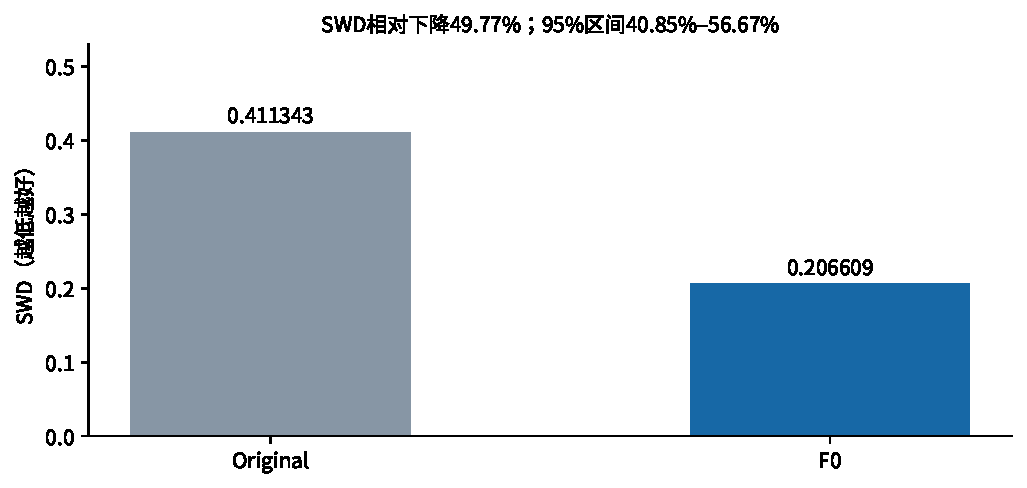
\includegraphics[width=0.90\textwidth]{figures/ch06/f0_swd_baseline.pdf}
 \caption{统一评价中Original与初始生成器的SWD对照。相对下降及区间均取自既有组Bootstrap记录，不代表完整迁移通过。}
 \label{fig:ch06_f0_swd_baseline}
\end{figure}

多轮实验使用Real Train的5153窗、32个Session及Natural Train的4049窗、50个Root；外层Validation分别为780窗、4个Session和905窗、10个Root。判别器内部再划分Real fit的24个Session、4217窗与inner的8个Session、936窗，Natural fit的40个Root、3249窗与inner的10个Root、800窗。各轮沿用这一隔离；inner不参与D更新，但生成器可用全部Natural Train，因此它不是生成器独立测试。外层Validation也已有开发暴露，以下结果均不称为盲测结论。

实验采用Seed 4901，固定Euler步数$K=1$，最多更新生成器三次。先以原始Real与Natural数据训练$D_0$，再用$F_0$输出继续适应同一判别器得到$D_1$；冻结$D_1$后更新原生成场为$F_1$。随后依次以$F_1$、$F_2$作为负类生成来源，得到$D_2$、$D_3$，并在各自冻结边界下更新为$F_2$、$F_3$。这些符号表示持续继承的模型状态，而非每次另建模型；Adam状态也连续保留。$D_0$训练20个Epoch、1320步，其后三个D阶段各10个Epoch、660步，累计3300步；每个G阶段20个Epoch、1280步，累计3840步。这里的三轮对抗优化与数值积分步数无关。

生成器继承A组终点，不意味着判别器也沿用连续输入配置。本实验重新建立全局Mask加连续幅值判别器，保留硬Mask输入不可导的限制，没有采用C组的判别器STE。两套VAE继续冻结，训练保留对抗、输入保持及修正场约束，教师权重为零；域内采用分组等权损失，区别于前述窗口均值训练。因而，本实验检验的是这一具体多轮配置，不能把结果归结为对所有梯度修复方案的验证。

执行中还发生了明确记录的协议修订。初始登记额外要求inner与fit的CE差不超过0.2，在$D_1$完成、$G_1$开始前触发停止。2026年11月19日经授权，将该差距改为诊断项，保留原停止记录，从已有$D_1/F_0$及对应Adam状态继续，不重训$D_1$，也不重置预算。复核得到$D_1$ inner BA约0.924151、AUC约0.969299，但一个Real Session召回仅0.133333，说明宏观判别能力并不能掩盖组间薄弱环节。后续结果应视为保留修订记录的开发性诊断，而非始终未变更的预注册执行。

\begin{figure}[htbp]
 \centering
 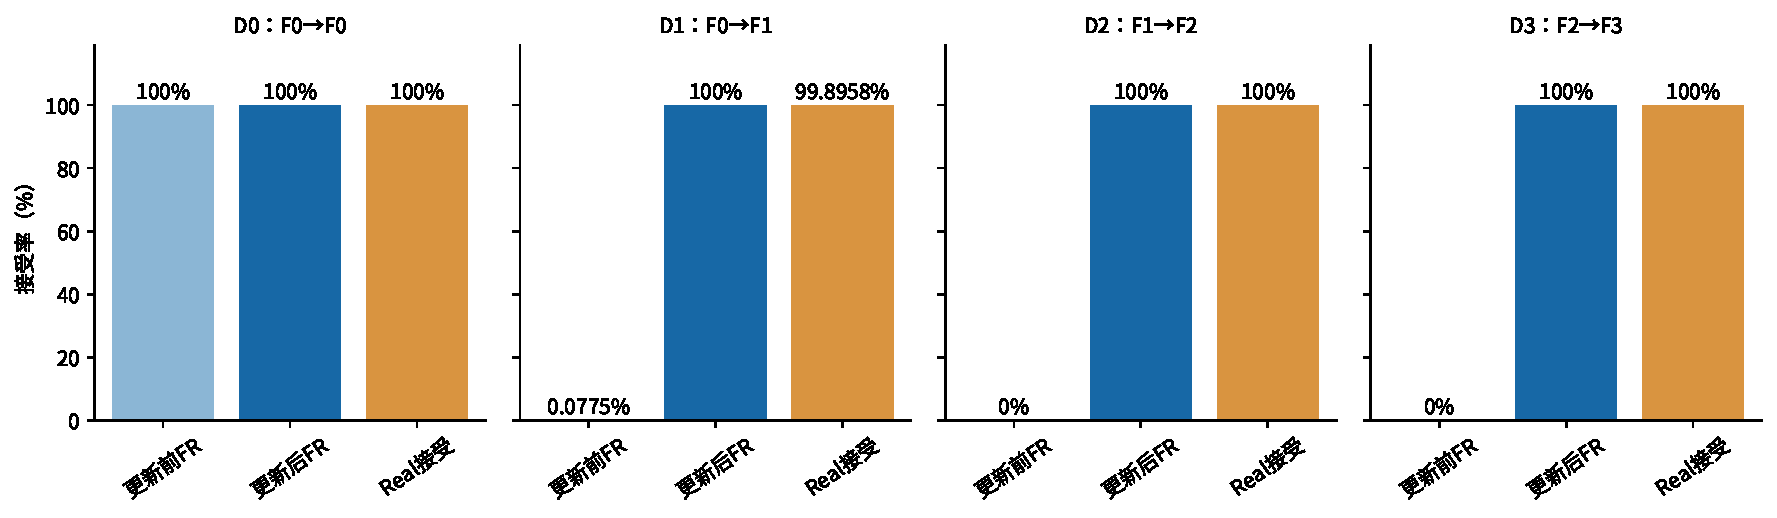
\includegraphics[width=\textwidth]{figures/ch06/round_acceptance_states.pdf}
 \caption{各判别器状态下生成器更新前后的接受率。每组仅在同一冻结D内比较；第0轮为原域判别器诊断，Real接受率按Session宏平均。}
 \label{fig:ch06_round_acceptance_states}
\end{figure}

FR定义为Sim生成样本被当前冻结判别器按0.5阈值判为Real的接受比例，先在Root内计算，再对10个Root宏平均；Real接受率先在Session内计算，再对4个Session宏平均，二者不是相同统计指标。如图\ref{fig:ch06_round_acceptance_states}所示，$F_0$在$D_0$下本来就达到100\% FR，不是生成器更新收益。$D_1$下$F_0\rightarrow F_1$的FR由约0.000775升至1，$D_2$下$F_1\rightarrow F_2$、$D_3$下$F_2\rightarrow F_3$均由0升至1。对应Real宏接受率分别约为0.998958、1和1。它们证明各次更新改变了当前判别边界下的输出判定；由于D已经改变，不能将各轮FR拼成同一评价器下的连续改善曲线。

\begin{figure}[htbp]
 \centering
 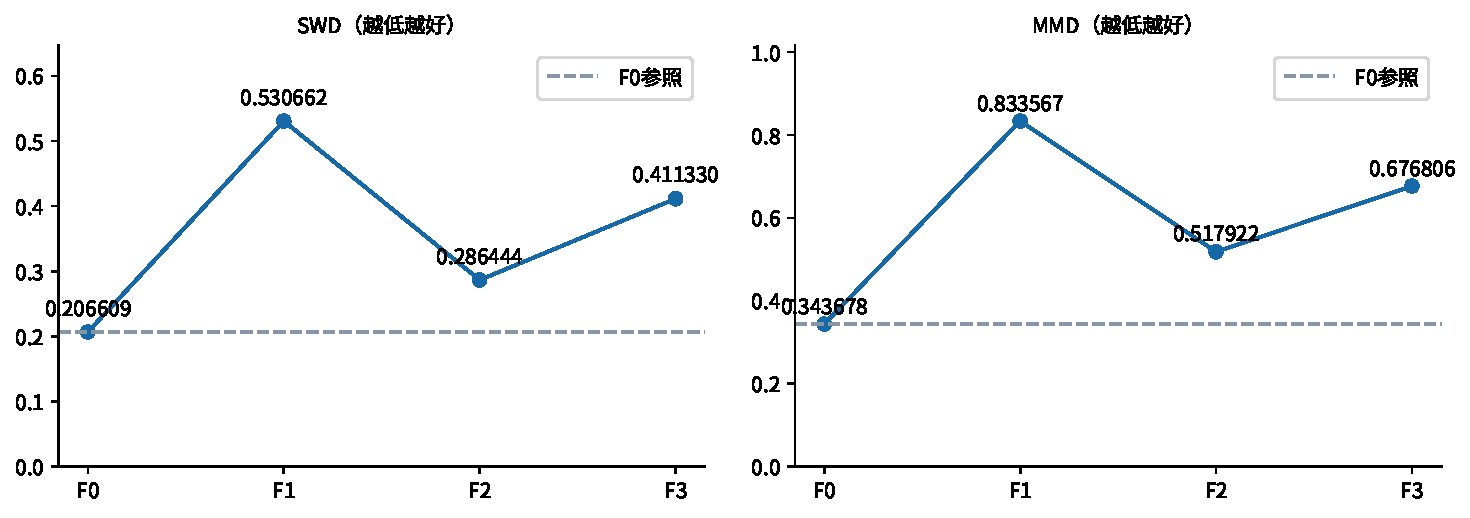
\includegraphics[width=\textwidth]{figures/ch06/multi_round_distribution.pdf}
 \caption{固定分布评价合同下各生成器状态的SWD与MMD。两项均越低越好，生成结果未随优化轮次单调改善。}
 \label{fig:ch06_multi_round_distribution}
\end{figure}

固定距离评价沿用相同Validation、Real Train预处理及冻结投影和核设置，不按各轮输出重新拟合参照。这一评价给出了不同判断。图\ref{fig:ch06_multi_round_distribution}中，$F_1$的SWD/MMD由$F_0$的0.206609/0.343678升至0.530662/0.833567，并在既有护栏中出现严重样本差异收缩。$F_2$恢复至0.286444/0.517922，仍未回到初始水平；$F_3$又反弹至0.411330/0.676806。同一P49合同下Original的SWD/MMD为0.411343/0.392554，故$F_3$的SWD已接近未转换输入，但MMD仍较高。终点两项距离均高于$F_0$，不能称为多轮质量持续提升，也不能把中间恢复忽略后描述成单调恶化。其中，跨窗口离散程度按2848个时序坐标的窗口间标准差再取均值计算，不作Root加权，并非物理接触多样性的认证指标。该量从约0.054778降至$F_1$的0.000201；905个Validation输出按完整窗口字节内容去重后仍有877种，但这种数值唯一性不能排除实际响应收缩。终点的分布、邻域覆盖、幅值及空间护栏仍未满足参照限制，部分时序项通过不能抵消这些不足。$F_0$作为相对非退化参照，并不因此获得完整质量认证。

更值得注意的是，$D_3$下$F_3$虽全部被判为Real，AUC仍约为0.997728。阈值判定只检查分数落在哪一侧，而AUC衡量连续分数将Real排在生成样本之前的能力；全部超过0.5仍可在阈值上方保持清晰排序，故两者不矛盾。AUC也不直接度量生成分布质量。因此，FR达到100\%并不等于域不可辨识，更不能替代原11实例C0联合评价。这些结果提示生成场能够适应当前判别边界，但分布逼近及输入保持并未同时得到保证。单Seed、既有开发划分和保留的梯度限制也约束了归因范围，后续需要进一步检查生成结构与评价器可靠性，而非仅增加优化轮数。
